\documentclass[conference]{IEEEtran}
\usepackage{cite}
\usepackage{amsmath,amssymb}
\usepackage{graphicx}
\usepackage{booktabs}
\usepackage{tikz}
\usetikzlibrary{arrows.meta,positioning}
\usepackage{url}
\usepackage[hidelinks]{hyperref}
\graphicspath{{figures/}}
\hypersetup{
  pdftitle={Memory-Based Malware Detection: Dataset Bias and Baseline-Differential Analysis},
  pdfauthor={Joel C. Okore, Andrei Petrovski, Igor V. Kotenko},
  pdfkeywords={memory forensics, malware detection, dataset bias, baseline modeling}
}

\begin{document}

\title{Memory-Based Malware Detection:\\
Dataset Bias and Baseline-Differential Analysis}

\author{\IEEEauthorblockN{Joel C. Okore}
\IEEEauthorblockA{\textit{Faculty of Computer Science} \\
\textit{Innopolis University}\\
Innopolis, Tatarstan, Russia \\
j.okore@innopolis.university}
\and
\IEEEauthorblockN{Andrei Petrovski}
\IEEEauthorblockA{\textit{Faculty of Computer Science} \\
\textit{Innopolis University}\\
Innopolis, Tatarstan, Russia \\
a.petrovski@innopolis.ru}
\and
\IEEEauthorblockN{Igor V. Kotenko}
\IEEEauthorblockA{\textit{Security Problems Lab} \\
\textit{SPC RAS}\\
St. Petersburg, Russia \\
ivkote@comsec.spb.ru}
\IEEEauthorblockA{\textit{Institute of Information Security} \\
\textit{Innopolis University}\\
Innopolis, Tatarstan, Russia \\
i.kotenko@innopolis.ru}}

\maketitle

\begin{abstract}
Memory forensics supports malware investigation by exposing process and memory
artifacts that may be unavailable in disk-based evidence. Integrating this
analysis into automated incident response requires classifiers whose decisions
remain meaningful across host configurations and workloads. In this work, we
present a memory-forensics pipeline combining Wazuh, WinPMEM, Volatility3, and
machine-learning-based response, and examine the reliability of its training
data. An audit of CIC-MalMem-2022 shows that six host-configuration features
achieve 99.98\% accuracy under a random split, compared with 99.99\% using all
nonconstant features. A single-service-count rule achieves 99.63\% on the full
corpus, while class-conditional feature distributions exhibit limited overlap.
These findings, together with the documented collection and oversampling
procedures, indicate that benchmark accuracy alone does not establish sensitivity
to malicious behavior. We propose a baseline-differential representation that
measures deviations from clean reference captures of the same host. A pilot
using five process-injection sub-techniques provides six retained pre/post pairs
and identifies a persistent baseline shift in four subsequent trials. The
retained pairs show test-associated changes in injection and module features,
but none exceeds the restricted scorer's default alert threshold. The results
support further evaluation of host-relative memory analysis and show why baseline
integrity and independent calibration are necessary before automated containment.
\end{abstract}

\begin{IEEEkeywords}
memory forensics, malware detection, dataset bias, baseline modeling,
incident response, security automation
\end{IEEEkeywords}

\section{Introduction}

Memory forensics provides evidence about processes, modules, services, and
executable memory regions relevant to malware investigation. These artifacts
can disappear as processes terminate or memory is reused. Security Information
and Event Management (SIEM) platforms can initiate acquisition when endpoint
activity satisfies a detection rule, helping preserve evidence for analysis.

Machine learning can extend this workflow by classifying memory features and
triggering automated response. However, process, service, and handle counts
reflect host configuration and workload as well as potentially malicious
activity. A model can therefore distinguish benchmark classes using differences
that do not transfer to another endpoint, a recurring evaluation concern in
security machine learning~\cite{arp2022}.

We investigate this issue through an automated pipeline integrating Wazuh active
response, WinPMEM acquisition, Volatility3 analysis, and an XGBoost classifier.
The original system was demonstrated in an isolated WannaCry experiment. Its
classifier used two service-related features from CIC-MalMem-2022~\cite{carrier2022}
and achieved approximately 99.8\% accuracy in the original training experiment.
This result motivated an examination of whether the benchmark separates
malicious behavior from the conditions under which memory was collected.

Our analysis finds high accuracy using host-configuration features alone and
limited class overlap at similar system load. These observations motivate
assessing each capture against clean references from the same endpoint. This
host-relative representation reduces dependence on absolute counters while
retaining the need to account for workload and reference-state changes.

The contributions of this work are as follows:
\begin{enumerate}
\item An automated memory-forensics workflow connecting SIEM alerts, memory
acquisition, feature extraction, classification, and containment, demonstrated
with live ransomware in a virtualized testbed.
\item An audit of CIC-MalMem-2022 using feature-group ablation, class-conditional
distributions, overlap analysis, and the published collection methodology.
\item A baseline-differential representation fitted using clean captures from
the same host, with an explicit robust deviation score.
\item A paired attack-emulation pilot examining feature changes, score
sensitivity, and baseline contamination during sequential collection.
\end{enumerate}

\section{Related Work}

VolMemLyzer~\cite{lashkari2021} extracts memory features for malware
classification. Carrier et al.~\cite{carrier2022} extended this approach with
obfuscation-related features and introduced CIC-MalMem-2022, reporting 99.00\%
accuracy and a 99.02\% F1-score for their stacked ensemble. The benchmark
contains features derived from processes, modules, services, and other memory
artifacts~\cite{carrier2022}. These support comparisons between learning methods,
but deployment also requires evidence that the learned relationships persist
under different collection conditions.

Wazuh supports active-response scripts triggered by alert rules, levels, or
groups~\cite{wazuh}. This mechanism can connect endpoint detection to
acquisition and containment. Volatility3 supplies the memory-analysis
components, including heuristics for identifying potentially injected memory
regions~\cite{volatility3}. Our system integrates these capabilities into an
event-driven forensic workflow and uses the resulting deployment context to
examine the validity of the classifier's inputs.

Arp et al.~\cite{arp2022} describe sampling bias, data leakage, and evaluation
pitfalls in security machine learning. We apply these concerns to a public
memory-forensics benchmark and evaluate a host-relative alternative in a
paired experiment. The audit examines between-class separation; the pilot
examines within-host changes after attack emulation.

\section{System Architecture}
\label{sec:architecture}

The original testbed comprises a Windows 10 endpoint and an Ubuntu Wazuh manager.
The endpoint runs the Wazuh agent and WinPMEM. The manager hosts detection
rules, active-response scripts, Volatility3, and the classifier.
Fig.~\ref{fig:architecture} summarizes the workflow.

\begin{figure}[t]
\centering
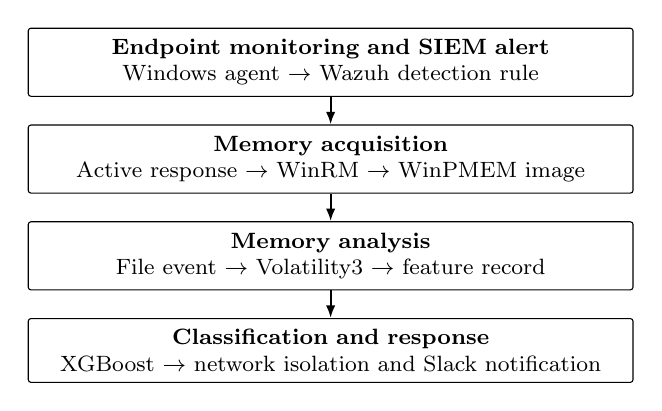
\begin{tikzpicture}[
  node distance=3.5mm,
  stage/.style={draw,rounded corners=1pt,align=center,
    text width=7.4cm,inner sep=4pt,font=\footnotesize},
  flow/.style={-{Latex[length=1.6mm]},thick}]
\node[stage] (alert) {\textbf{Endpoint monitoring and SIEM alert}\\
Windows agent $\rightarrow$ Wazuh detection rule};
\node[stage,below=of alert] (capture) {\textbf{Memory acquisition}\\
Active response $\rightarrow$ WinRM $\rightarrow$ WinPMEM image};
\node[stage,below=of capture] (features) {\textbf{Memory analysis}\\
File event $\rightarrow$ Volatility3 $\rightarrow$ feature record};
\node[stage,below=of features] (model) {\textbf{Classification and response}\\
XGBoost $\rightarrow$ network isolation and Slack notification};
\draw[flow] (alert) -- (capture);
\draw[flow] (capture) -- (features);
\draw[flow] (features) -- (model);
\end{tikzpicture}
\caption{Original automated memory-forensics pipeline. The baseline-differential
scorer is evaluated separately as a candidate replacement for the classifier.}
\label{fig:architecture}
\end{figure}

\subsection{Detection and Memory Acquisition}
Custom Wazuh rules monitor PowerShell operational logs for indicators such as
encoded commands and known offensive cmdlets. An alert at severity level 10 or
above invokes an active-response script. The script uses NetExec over Windows
Remote Management (WinRM) to launch WinPMEM on the endpoint and write a raw
memory image to a location accessible to the manager.

\subsection{Feature Extraction and Automated Response}
File-integrity monitoring on the dump path initiates feature extraction.
The original extractor runs Volatility3's service scan and produces two
features: the number of service records and the number of distinct nonzero
process identifiers associated with those records. A subsequent file event
invokes the classifier. A malicious prediction triggers a remote command to
disable the endpoint's network adapters and a Slack notification containing the host
and model output.

The original WannaCry experiment exercised acquisition, feature extraction,
classification, and response. The retained logs record 171\,s from the start
of the acquisition script to the start of the response script. They do not
provide a separate containment-completion timestamp, so this interval describes
workflow progression rather than a measured end-to-end containment latency.
The experiment establishes that the components can operate together; classifier
generalization is examined separately below.

\section{Dataset Audit}
\label{sec:diagnosis}

CIC-MalMem-2022 contains 58{,}596 records, with 29{,}298 records in each class
and 55 numeric memory features~\cite{carrier2022,cicmalmem}. The audit excludes
the class and category fields from model inputs and removes three constant
features, leaving 52 predictors. We examine feature-group performance, effect
directions, and distributional overlap to assess how readily host-state
differences can explain the observed discrimination.

\subsection{Feature-Group Ablation and Threshold Baseline}
The ablation uses a stratified 70/30 train/test split with random seed 7.
Each XGBoost model uses 200 estimators and a maximum depth of 6, with feature
scaling fitted on the training partition. The feature groups comprise all
52 nonconstant predictors, six service/driver/module/callback counters,
24 features from the \texttt{malfind}, \texttt{ldrmodules}, and
\texttt{psxview} families, and the two service features used by the original
pipeline.

Table~\ref{tab:ablation} reports the results. The six host-configuration
features achieve 99.98\% accuracy, compared with 99.99\% for the full
nonconstant feature set. The two-service-feature model achieves 99.84\%.
As a descriptive baseline, the rule
\begin{equation}
\hat{y}=\mathbf{1}\{\texttt{nservices}\leq391\ \lor\
                         \texttt{nservices}>1000\}
\end{equation}
achieves 99.63\% on the full corpus. This rule uses one feature and no fitted
classifier. Its corpus-level result is not an independent held-out estimate,
but shows that a simple service-count boundary reproduces much of the observed
class separation.

\begin{table}[t]
\caption{Feature-Group Accuracy on CIC-MalMem-2022}
\label{tab:ablation}
\centering
\small
\begin{tabular}{@{}lrr@{}}
\toprule
Feature group & Features & Accuracy (\%) \\
\midrule
All nonconstant features & 52 & 99.99 \\
Host-configuration counters & 6 & 99.98 \\
Injection/hiding features & 24 & 99.98 \\
Two service features & 2 & 99.84 \\
Service-count rule$^{\ast}$ & 1 & 99.63 \\
\bottomrule
\end{tabular}
\par\smallskip
\begin{minipage}{\columnwidth}\footnotesize
Models use the same stratified 70/30 split. $^{\ast}$The fixed rule is evaluated
on the full corpus and has no fitted classifier parameters.
\end{minipage}
\end{table}

\subsection{Class-Conditional Feature Distributions}
All 22 count and count-derived features selected by the direction audit have
higher benign medians. This selected set includes process, service, handle,
module, and injection-related measures; it is not an exhaustive inventory of
all counters. For example, the benign and malicious medians are 4 and 3 for
\texttt{malfind.ninjections}, and 74 and 46 for
\texttt{ldrmodules.not\_in\_load}. These directions show that higher absolute
values of injection-related counters cannot be interpreted as evidence of
infection without considering the reference environment.

Several benign configuration features also have little variation:
\texttt{svcscan.kernel\_drivers} takes three distinct values,
\texttt{svcscan.process\_services} four, and
\texttt{callbacks.ncallbacks} two across 29{,}298 benign records.
Together with the ablation, these observations are consistent with a strong
contribution from collection conditions and host state. They do not imply
that every feature is unrelated to malware.

\subsection{Feature-Space Overlap}
We estimate out-of-fold class probabilities
$e(x)=P(Y=\mathrm{malicious}\mid x)$ using five-fold cross-validation with
standardized logistic regression over the 52 nonconstant features. Only 0.92\%
of records lie in the intermediate band $0.1<e(x)<0.9$; the remaining
99.08\% receive probabilities outside this band
(Fig.~\ref{fig:overlap}). This is a diagnostic of strongly polarized class predictions
in the measured feature space. Because the inputs include potentially
malware-related features and do not directly identify capture conditions,
the statistic does not isolate the causal contribution of the collection
protocol.

The handle-count distributions provide a complementary view. The benign
5th percentile is 10{,}350, exceeding the malicious 95th percentile of
9{,}111. One-to-one matching within the load bins used by the audit retains
148 records, or 74 per class. The small matched subset limits comparisons
between records with similar measured load and supports caution about
transfer to other environments.

\begin{figure*}[t]
\centering
\includegraphics[width=\textwidth]{feature_overlap.pdf}
\caption{Distributional diagnostics for CIC-MalMem-2022. (a) Out-of-fold
malicious-class probabilities from logistic regression. (b) Handle-count
histograms with common logarithmically spaced bins, retaining all records and
using logarithmic axes. (c) Features with the smallest histogram-intersection overlap.}
\label{fig:overlap}
\end{figure*}

\subsection{Collection and Oversampling}
Carrier et al.~\cite{carrier2022} describe malicious execution in a Windows 10
VirtualBox VM with 2\,GB of memory and benign collection during normal
application use. They also report running benign applications during malicious
collection to reduce trivial process-based discrimination. The released table
provides insufficient capture-level provenance to reconstruct configuration
and workload differences between the classes. The observed feature differences
are consistent with class-associated host state, while their precise
collection-level cause remains unresolved.

The methodology reports balancing the benign class with Synthetic Minority
Over-sampling Technique (SMOTE) during dataset construction~\cite{carrier2022}.
In the local dataset, \texttt{malfind.uniqueInjections} has 209 distinct
malicious values and 5{,}337 distinct benign values. The dense fractional benign
values are consistent with interpolation. Splitting this released table at
random can therefore place related original and synthetic observations across
partitions. Without original-capture identifiers and interpolation provenance,
the extent of such dependence cannot be quantified. This risk is separate
from the limited feature-distribution overlap and further constrains the
interpretation of random-split accuracy.

\section{Baseline-Differential Method}
\label{sec:method}

The proposed representation measures a candidate capture's deviation from clean
references of the same host. Fitting requires only clean captures; independent
benign and attack captures are needed for evaluation and calibration.

\subsection{Feature Representation and Score}
The pilot extractor aggregates 44 features from eight Volatility3 plugins:
process listing, DLL listing, handles, loader modules, suspicious memory
regions, kernel modules, services, and callbacks. These are locally defined
aggregates; shared names do not establish equivalence with the original
55-feature benchmark schema.

For clean reference set $C$, let $m_i$ be the median of feature $i$ and
$d_i=1.4826\,\operatorname{median}_{c\in C}|c_i-m_i|$ its scaled median
absolute deviation. The implemented scale is
\begin{equation}
s_i=\begin{cases}
\max(0.01|m_i|,1), & d_i<10^{-6},\\
d_i, & \text{otherwise}.
\end{cases}
\end{equation}
The fallback prevents division by a near-zero scale for features that are
effectively constant in the reference set. Each candidate feature is represented
by a robust deviation and a companion ratio:
\begin{equation}
z_i(x)=\frac{x_i-m_i}{s_i+\epsilon},\qquad
r_i(x)=\frac{x_i+1}{m_i+1},\quad \epsilon=10^{-9}.
\end{equation}
The ratio aids interpretation; the implemented alert score uses deviations:
\begin{equation}
S_F(x)=\max_{i\in F}|z_i(x)|.
\label{eq:score}
\end{equation}
The implementation also reports the mean absolute standardized deviation and the number of
features with $|z_i|>3$. Its default alert threshold is $S_F(x)\geq6$.
This threshold is an implementation setting and has not been calibrated as an
operating point for the pilot.

We examine both the full 44-feature set and an exploratory restriction to the
11 \texttt{malfind} and \texttt{ldrmodules} features. For the pilot, each
reference model is fitted to the six retained pre-test captures. Scores on
these same references describe the fit and do not estimate an independent
false-positive rate. Paired feature differences
$\Delta x_i=x_i^{\mathrm{post}}-x_i^{\mathrm{pre}}$ provide a complementary
description that does not depend on the score threshold.

\subsection{Paired Collection Protocol}
Each trial obtains a pre-test capture, invokes attack emulation, and obtains
a post-test capture on the same VM. Workloads vary between trials while the
host image remains fixed. Pairing controls host identity, but background
activity and residual state can still vary. Reference collection therefore
requires representative workloads and verification of baseline integrity.

\section{Pilot Evaluation and Discussion}
\label{sec:evaluation}

\subsection{Experimental Setup}
The pilot uses a Google Cloud \texttt{e2-medium} VM running Windows Server 2022
and Atomic Red Team~\cite{atomicredteam} tests associated with five MITRE
ATT\&CK process-injection sub-techniques~\cite{mitre1055}: DLL injection
(T1055.001), portable executable injection (T1055.002), thread execution
hijacking (T1055.003), asynchronous procedure call (APC) injection (T1055.004),
and process hollowing (T1055.012). These tests exercise attack mechanisms
without constituting full malware executions.

Ten trials were collected sequentially within one boot session, with
process-level and Atomic Red Team cleanup between trials. The script cycles
through five workload labels. The \texttt{browser} label launches Notepad and
Paint; \texttt{office} launches Notepad, Calculator, and Explorer;
\texttt{mixed} launches Notepad, Paint, and Calculator; and \texttt{busy}
starts four compute-bound PowerShell processes. These labels identify
lightweight application profiles, rather than measured browsing or office
sessions. Technique and workload follow the same fixed rotation, so their
effects cannot be estimated independently.

We use \emph{pre-test} and \emph{post-test} for the records labeled
\texttt{clean} and \texttt{infected} in the collection files. The labels
denote acquisition order relative to emulation; they do not independently
verify that every requested test succeeded.

\subsection{Baseline Integrity}
Inspection of the feature trajectories revealed a persistent shift beginning
with trial 7. The aggregate \texttt{malfind.commitCharge} value increased from
259--265 in the pre-test captures of trials 1--6 to 773--778 in the pre-test
captures of trials 7--10 (Table~\ref{tab:contamination}). The elevated state
continued through the remaining post-test captures. The first six pairs are
retained for the quantitative analysis; the final four are reported as an
observed baseline-contamination episode.

\begin{table}[t]
\caption{Observed Baseline Shift in Sequential Collection}
\label{tab:contamination}
\centering
\small
\begin{tabular}{@{}lcc@{}}
\toprule
Trials & Pre-test commit charge & All captures \\
\midrule
1--6 & 259--265 & 259--272 \\
7--10 & 773--778 & 773--778 \\
\bottomrule
\end{tabular}
\end{table}

The approximately threefold change is consistent with residual memory state
after incomplete cleanup. The aggregate records establish its timing and
persistence within the session, but do not identify the responsible process
or prove attribution to a particular injection. The episode shows that
same-host pairing alone is insufficient to preserve a clean reference during
sequential tests. Future collection should restore a known-clean snapshot
between trials and verify the baseline before acquisition.

\subsection{Paired Feature Changes}
Table~\ref{tab:deltas} reports the post-minus-pre differences for the six
retained pairs. The loader-module counts increase in five pairs and decrease
by two in the T1055.002 pair. Injection-region and commit-charge counts either
increase or remain unchanged. The APC-injection and process-hollowing pairs
show increases across all four reported features; three of the other four
pairs have unchanged \texttt{malfind} values.

\begin{table}[t]
\caption{Post-Test Minus Pre-Test Feature Values ($n=6$ Pairs)}
\label{tab:deltas}
\centering
\small
\setlength{\tabcolsep}{3pt}
\begin{tabular}{@{}lrrrr@{}}
\toprule
Technique (workload label) & $\Delta I$ & $\Delta C$ & $\Delta L$ & $\Delta M$ \\
\midrule
T1055.001 (idle) & $+1$ & $+2$ & $+1$ & $+1$ \\
T1055.002 (browser) & $0$ & $0$ & $-2$ & $-2$ \\
T1055.003 (office) & $0$ & $0$ & $+1$ & $+1$ \\
T1055.004 (mixed) & $+3$ & $+3$ & $+15$ & $+15$ \\
T1055.012 (busy) & $+1$ & $+7$ & $+5$ & $+5$ \\
T1055.001 (idle, repeat) & $0$ & $0$ & $+21$ & $+21$ \\
\bottomrule
\end{tabular}
\par\smallskip
\begin{minipage}{\columnwidth}\footnotesize\raggedright
$I$: \texttt{malfind.ninjections}; $C$: \texttt{malfind.commitCharge};
$L$: \texttt{ldrmodules.not\_in\_load};
$M$: \texttt{ldrmodules.not\_in\_mem}.
\end{minipage}
\end{table}

These observations should be interpreted in relation to the extraction
heuristics. Volatility3's \texttt{malfind} examines memory-region properties
such as protection, backing, and page contents~\cite{volatility3}; it is not a
complete detector for every implementation of process injection. The observed
variation is compatible with sensitivity to the memory regions created by a
test. However, technique identifiers and aggregate counts alone do not
establish the exact allocation mechanism or a general detectability boundary
for an ATT\&CK sub-technique.

\subsection{Score Behavior and Operational Implications}
With the restricted 11-feature representation, pre-test maximum-deviation
scores range from 0.678 to 4.000 and post-test scores from 0.703 to 5.000.
The APC-injection pair increases from 0.797 to 3.000, and the process-hollowing
pair from 4.000 to 5.000. Thus, both pairs move upward under the proposed
score, but neither crosses the default threshold of 6. No retained pre-test
or post-test capture exceeds that threshold. This is evidence of relative
feature changes, rather than successful threshold-based detection.

Using all 44 features produces alerts on three post-test captures and one
reference capture, with the reference alert driven by \texttt{handles.nkey}
in the busy workload. Restricting the features removes
that alert on the same fitted references, but this in-sample comparison cannot
establish specificity. It illustrates the sensitivity of a maximum-deviation
score to feature choice and limited baseline coverage. In an automated response
pipeline, independent calibration across clean workloads is required before
such scores can justify host isolation.

\section{Limitations}
\label{sec:limitations}

The observational audit lacks the capture-level provenance needed to separate
host configuration, workload, oversampling, and malicious execution as causes.
It identifies threats to benchmark interpretation, without estimating
deployment error rates.

The pilot contains six retained pairs from one host image, with coupled
workloads and techniques. Excluding the visible baseline shift does not rule
out earlier residual effects. The collection script removes raw images after
extraction, and per-test execution transcripts are unavailable in the retained
artifacts. This limits retrospective validation of test success and individual
memory mechanisms.

The clean references are also reused for score assessment, and the feature
restriction is exploratory. Larger independent reference and evaluation sets
are required to estimate false-positive and detection rates and to select an
alert threshold. Finally, the WannaCry demonstration predates the proposed
representation. The baseline-differential scorer has not yet been validated
against full malware executions or integrated into the automated containment
path.

\section{Conclusion}

This work presents an automated memory-forensics pipeline and examines the
reliability of the benchmark used to train its classifier. In CIC-MalMem-2022,
host-configuration features achieve accuracy close to the full nonconstant
feature set, while class-conditional distributions show limited overlap.
Combined with the documented use of oversampling, these findings motivate
evaluation beyond random splits of the released feature table.

The proposed baseline-differential representation measures deviations from
the same host's clean reference state. The pilot identifies baseline integrity
and workload coverage as central requirements for host-relative memory analysis.
Future work will use snapshot-isolated trials, independently varied workloads,
multiple host images, and full malware executions. Independent calibration
remains necessary before integrating the score into automated response.

\begin{thebibliography}{10}
\bibitem{arp2022} D. Arp, E. Quiring, F. Pendlebury, A. Warnecke,
F. Pierazzi, C. Wressnegger, L. Cavallaro, and K. Rieck,
``Dos and Don'ts of Machine Learning in Computer Security,'' in
\textit{Proc. 31st USENIX Security Symp.}, 2022, pp. 3971--3988.

\bibitem{carrier2022} T. Carrier, P. Victor, A. Tekeoglu, and A. H. Lashkari,
``Detecting Obfuscated Malware using Memory Feature Engineering,'' in
\textit{Proc. 8th Int. Conf. Information Systems Security and Privacy
(ICISSP)}, 2022, pp. 177--188, doi: 10.5220/0010908200003120.

\bibitem{lashkari2021} A. H. Lashkari, B. Li, T. L. Carrier, and G. Kaur,
``VolMemLyzer: Volatile Memory Analyzer for Malware Classification using
Feature Engineering,'' in \textit{Proc. Reconciling Data Analytics,
Automation, Privacy, and Security: A Big Data Challenge (RDAAPS)},
2021, pp. 1--8, doi: 10.1109/RDAAPS48126.2021.9452028.

\bibitem{wazuh} Wazuh, ``Active Response,'' \textit{Wazuh Documentation}.
Accessed: Sep. 9, 2026. [Online]. Available:
\url{https://documentation.wazuh.com/current/user-manual/capabilities/active-response/index.html}

\bibitem{volatility3} Volatility Foundation,
``volatility3.plugins.windows.malware.malfind,''
\textit{Volatility 3 Documentation}.
Accessed: Sep. 9, 2026. [Online]. Available:
\url{https://volatility3.readthedocs.io/en/latest/_modules/volatility3/plugins/windows/malware/malfind.html}

\bibitem{cicmalmem} Canadian Institute for Cybersecurity,
``Malware Memory Analysis (CIC-MalMem-2022),'' University of New Brunswick.
Accessed: Sep. 9, 2026. [Online]. Available:
\url{https://www.unb.ca/cic/datasets/malmem-2022.html}
\bibitem{atomicredteam} Red Canary, ``Atomic Red Team.''
Accessed: Sep. 9, 2026. [Online]. Available:
\url{https://github.com/redcanaryco/atomic-red-team}

\bibitem{mitre1055} MITRE, ``Process Injection, Technique T1055,''
\textit{MITRE ATT\&CK}.
Accessed: Sep. 9, 2026. [Online]. Available:
\url{https://attack.mitre.org/techniques/T1055/}

\end{thebibliography}
\end{document}
